In diesem Kapitel werden die Ergebnisse des vorher erläuterten Systems und den unterschiedlichen Architekturen faltender neuronaler Netze analysiert. An erster Stelle wird auf den Vorgang des Trainings eines neuronalen Netzes eingegangen. Darauffolgend werden die Netzwerkarchitekturen miteinander verglichen. Hierfür wurden drei unterschiedliche Vergleichsparameter festgelegt, auf welche näher eingegangen wird. Zudem werden mögliche Fehlerquellen betrachtet. Im Anschluss des Kapitels wird das System bewertet.


% Training
\section{Training}\label{sec:?}
In der Regel sieht der Trainingsverlauf eines neuronalen Netzes wie in Abbildung \ref{fig:vgg-verlaeufe} aus. Zu Beginn des Trainings liegt der Fehler auf einem hohen Wert, welcher innerhalb weniger Epochen stark gesenkt wird. Dabei werden die Verbesserungen im Verlauf immer kleiner, sodass diese Kurve abflacht und einen konvergenten Verlauf annimmt. Da sich der Fehler des Validierungsvorgangs ab einen bestimmten Zeitpunkt nicht mehr verbessert, wird das Training anhand des Early Stoppings angehalten. Die Anzahl an Epochen, die abgewartet werden, kann beliebig gewählt werden. Beispielsweise wurde dieser Wert im Verlauf des Trainings eines AlexNet, welcher in Abbildung \ref{fig:alexnet-log-scale} dargestellt ist, deutlich höher gesetzt, um die Auswirkungen des Overfittings zu zeigen. 

\begin{figure}[h!]
\centering
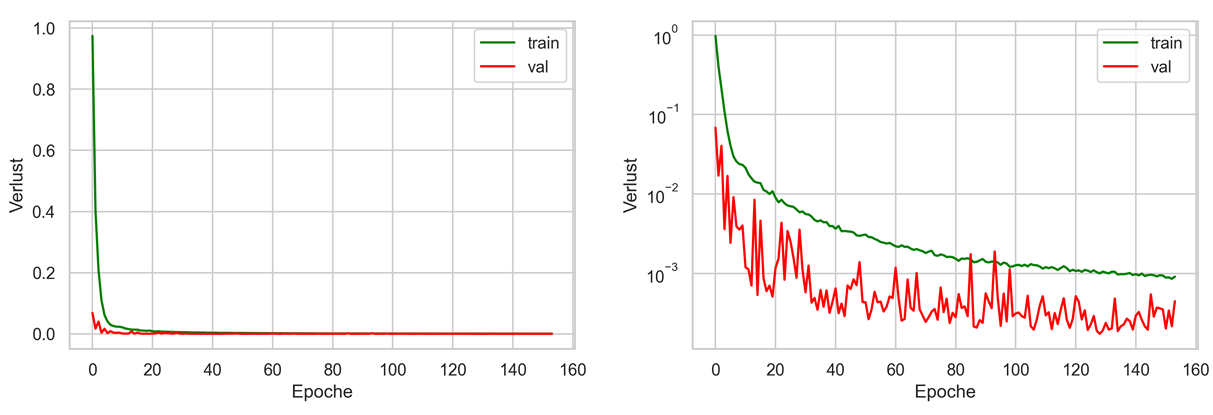
\includegraphics[width=16cm]{98_images/normal_log_vgg.png}
\caption{Verläufe des Trainingsvorgangs der VGG19-Architektur in linearer (links) und logarithmischer (rechts) Darstellung}
\label{fig:vgg-verlaeufe}
\end{figure}

\mypar Am logarithmischen Verlauf ist ebenfalls ersichtlich, dass das Netz bessere Ergebnisse in der Validierung als im Training erzielt. Dafür gibt es zwei Gründe. Zum einen wird das Dropout nicht im Validierungs- und Testvorgang angewendet, sondern nur während des Trainings. Zum anderen wird der Verlust im Training während den entsprechenden Epochen gemessen und aktualisiert. Im Gegensatz dazu wird der Validierungsfehler nach jeder Epoche berechnet, sodass die Parameter zu diesem Zeitpunkt auf angepassten Werten liegen.

\mypar Die Funktionsweise eines trainierten faltenden neuronalen Netzes kann mithilfe der Ausgaben aus den einzelnen Layern aufgezeigt werden. Ein vortrainiertes VGG19 erzeugt nach dem ersten Convolutional Layer 64 Feature Maps (siehe Abschnitt \ref{sec:vgg-sec}). Zehn die bei einer Eingabe des Bildes aus \ref{fig:30grad-cropped-img} entstandenen Feature Maps sind in Abbildung \ref{fig:activations-1} abgebildet.

\begin{figure}[h!]
\centering
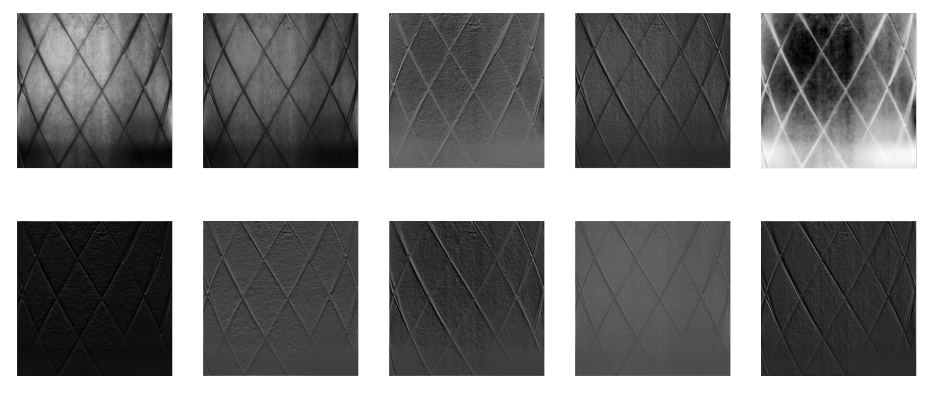
\includegraphics[width=12cm]{98_images/0_block1_conv1.png}
\caption{Zehn der 64 Feature Maps, welche durch das erste Convolutional Layer einer trainierten VGG19-Architektur entstehen}
\label{fig:activations-1}
\end{figure}

\mypar Durch die Anwendung der unterschiedlichen Filter aus dem Convolutional Layer werden die Kanten, also die Drähte des Stents, hervorgehoben. In den darauffolgenden Schritten wird die Dimensionalität der Eingabe durch die Anwendung weiterer Filter reduziert. Ebenso werden die Drähte im Bild verdeutlicht und der Hintergrund homogenisiert, wie in den Beispielen aus Abbildung \ref{fig:activations-2} gezeigt.

\begin{figure}[h!]
\centering
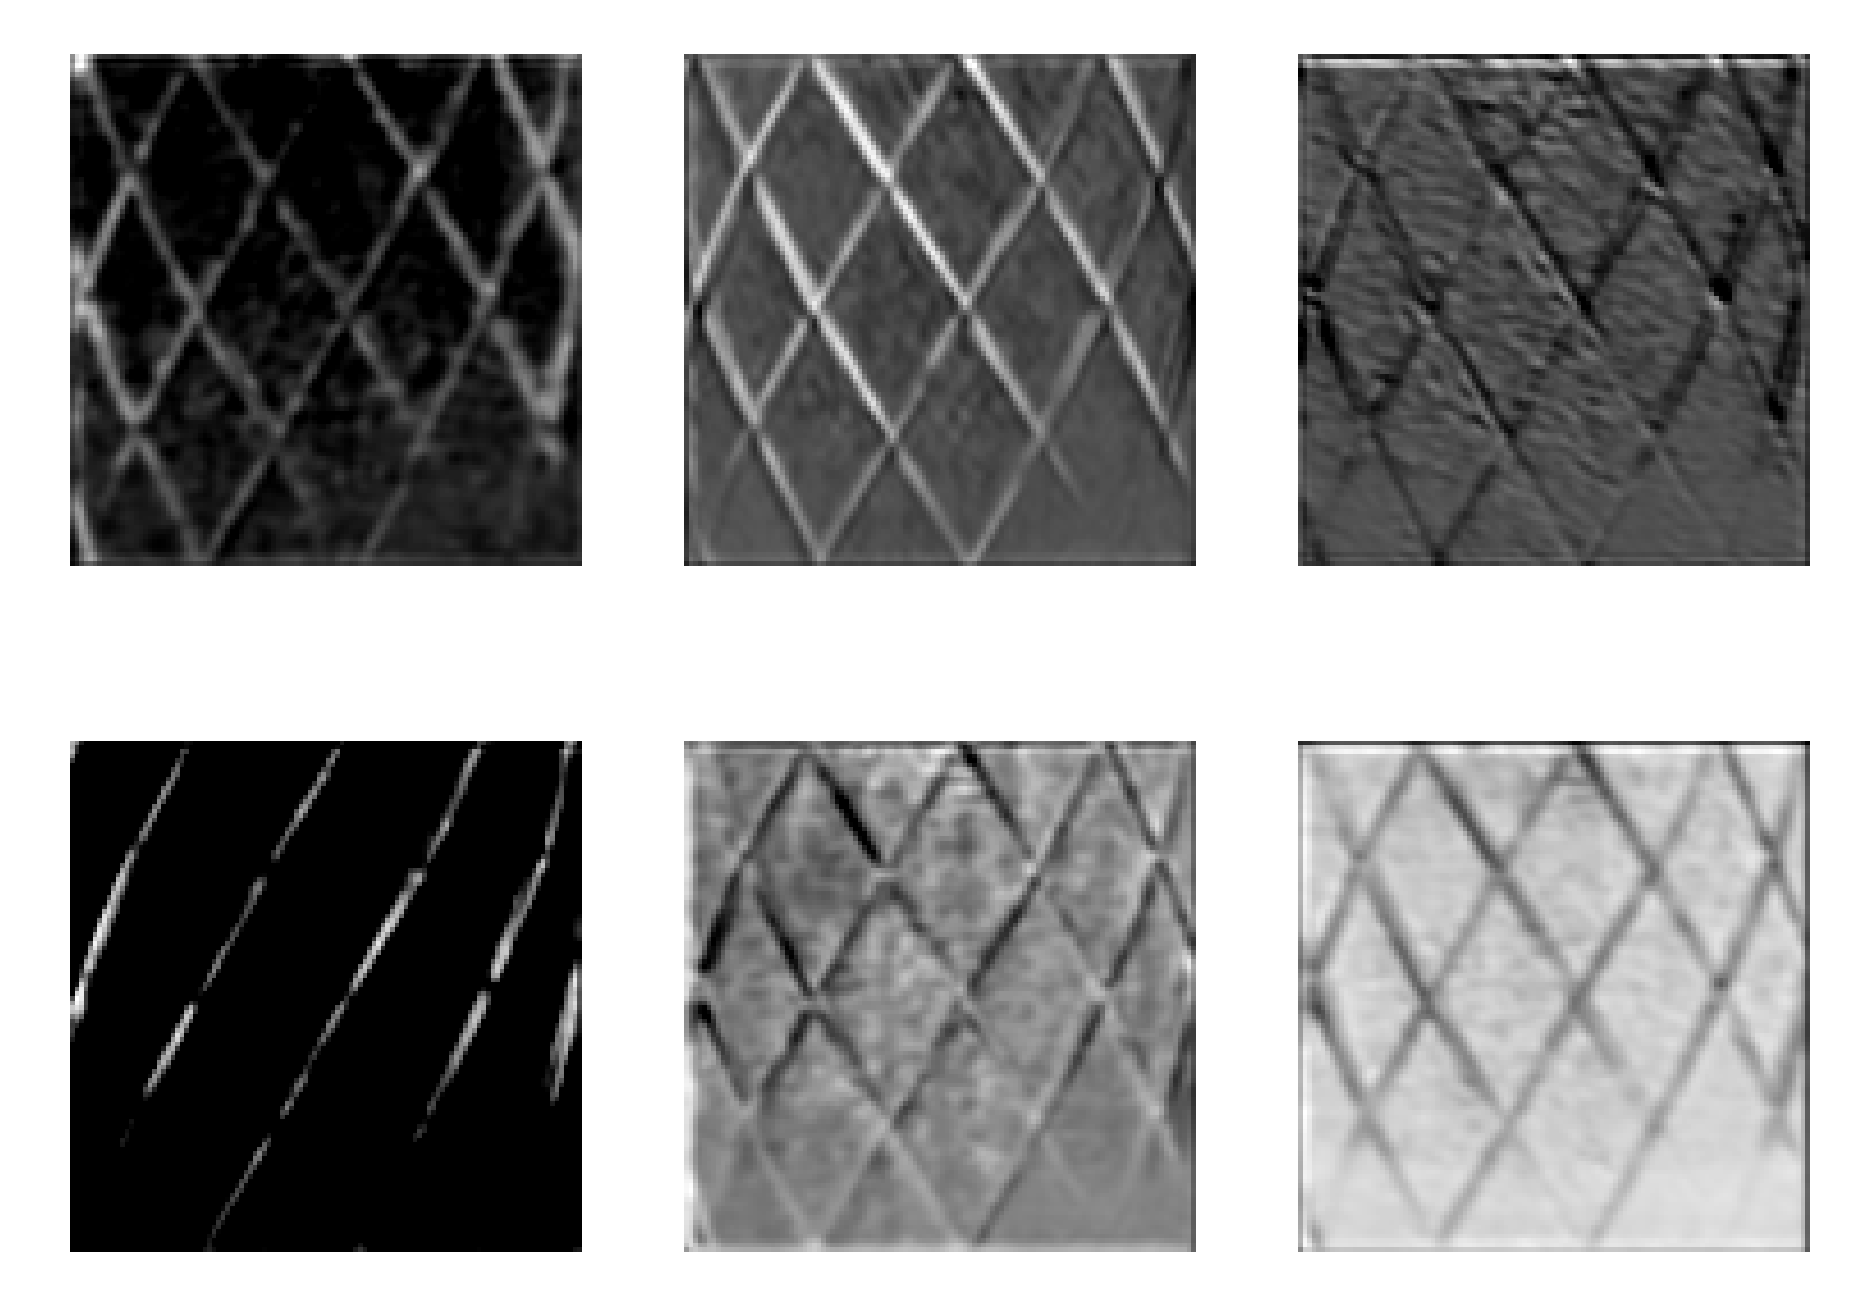
\includegraphics[width=7cm]{98_images/0_block3_conv4.png}
\caption{Sechs der 256 Feature Maps aus dem vierten und letzten Convolutional Layer im dritten Block des VGG19}
\label{fig:activations-2}
\end{figure}


% Bewertung der Ergebnisse
\section{Bewertung und Vergleich der Ergebnisse}
Insgesamt wurden drei grundlegende Vergleichsfaktoren gewählt: Der Fehler, welcher die durchschnittliche Abweichung zwischen der Netzausgabe und dem Soll-Wert darstellt, die benötigte Rechenzeit pro Bild und die gesamte Dauer des Trainings der Netze. Im Folgenden werden die Trainings- und Testergebnisse der einzelnen Netze miteinander bezüglich den zuvor genannten Faktoren verglichen. Eine Übersicht mit allen faltenden neuronalen Netzen und den Vergleichsgrößen wird in Anhang \ref{ch:Anhang-ch} in Tabelle \ref{Tab:vergleich-netze} aufgezeigt. 


% Fehler
\subsection{Fehler}\label{sec:fehler-sec}
Der Fehler ist das wichtigste Vergleichskriterium unter den neuronalen Netzen, da es sich auf die Genauigkeit dieser bezieht. Um Fehler möglichst richtig zu erkennen, muss das Netzwerk die Länge des Picks möglichst zuverlässig bestimmen können. 

\mypar Aus Abbildung \ref{fig:year-error-graph} kann abgelesen werden, dass das VGG19 in dieser Kategorie das beste Ergebnis erreicht. Die durchschnittliche Abweichung von 1,76 Pixel entpricht etwa 0,077 mm. Zudem schneidet das AlexNet, die älteste Architektur aus der Auswahl, mit Abstand am schlechtesten ab. Die neueste Architektur, das EfficientNet B2, erreicht in diesem Fall eine durchschnittliche Leistung bei 3,24 Pixel.


% Rechenzeit pro Bild
\subsection{Rechenzeit pro Bild}\label{sec:rechenzeit-label}
Als allgemeine Randbedingung wurde vorgegeben, dass das Gesamtsystem zur Fehlererkennung und -Korrektur in der Lage sein muss mindestens zehn Picks pro Sekunde zu inspizieren. Da das Bild durch alle Schichten der neuronalen Netze gespeist werden muss, hat die Anzahl an Schichten einen Einfluss auf die Dauer dieses Vorgangs. Abbildung \ref{fig:year-time-graph} zeigt die benötige Rechenzeit für ein Bild je Netz, wobei diese nach dem Veröffentlichungsjahr sortiert sind. Das AlexNet besitzt die niedrigste Anzahl an Schichten (sieben) und analysiert Bilder am schnellsten. Im Gegensatz dazu ist das Inception-ResNet-v2 das tiefste Netz und verbraucht die meiste Zeit zur Analyse. Trotz dieser Korrelation und des Einflusses der Anzahl an Schichten auf die Rechenzeit, sind beide Werte nicht proportional zueinander. Trotz der zweitniedrigsten Anzahl an Schichten verbraucht beispielsweise das VGG16 viel Zeit für die Analyse der Picklänge.

\begin{figure}[h!]
\centering
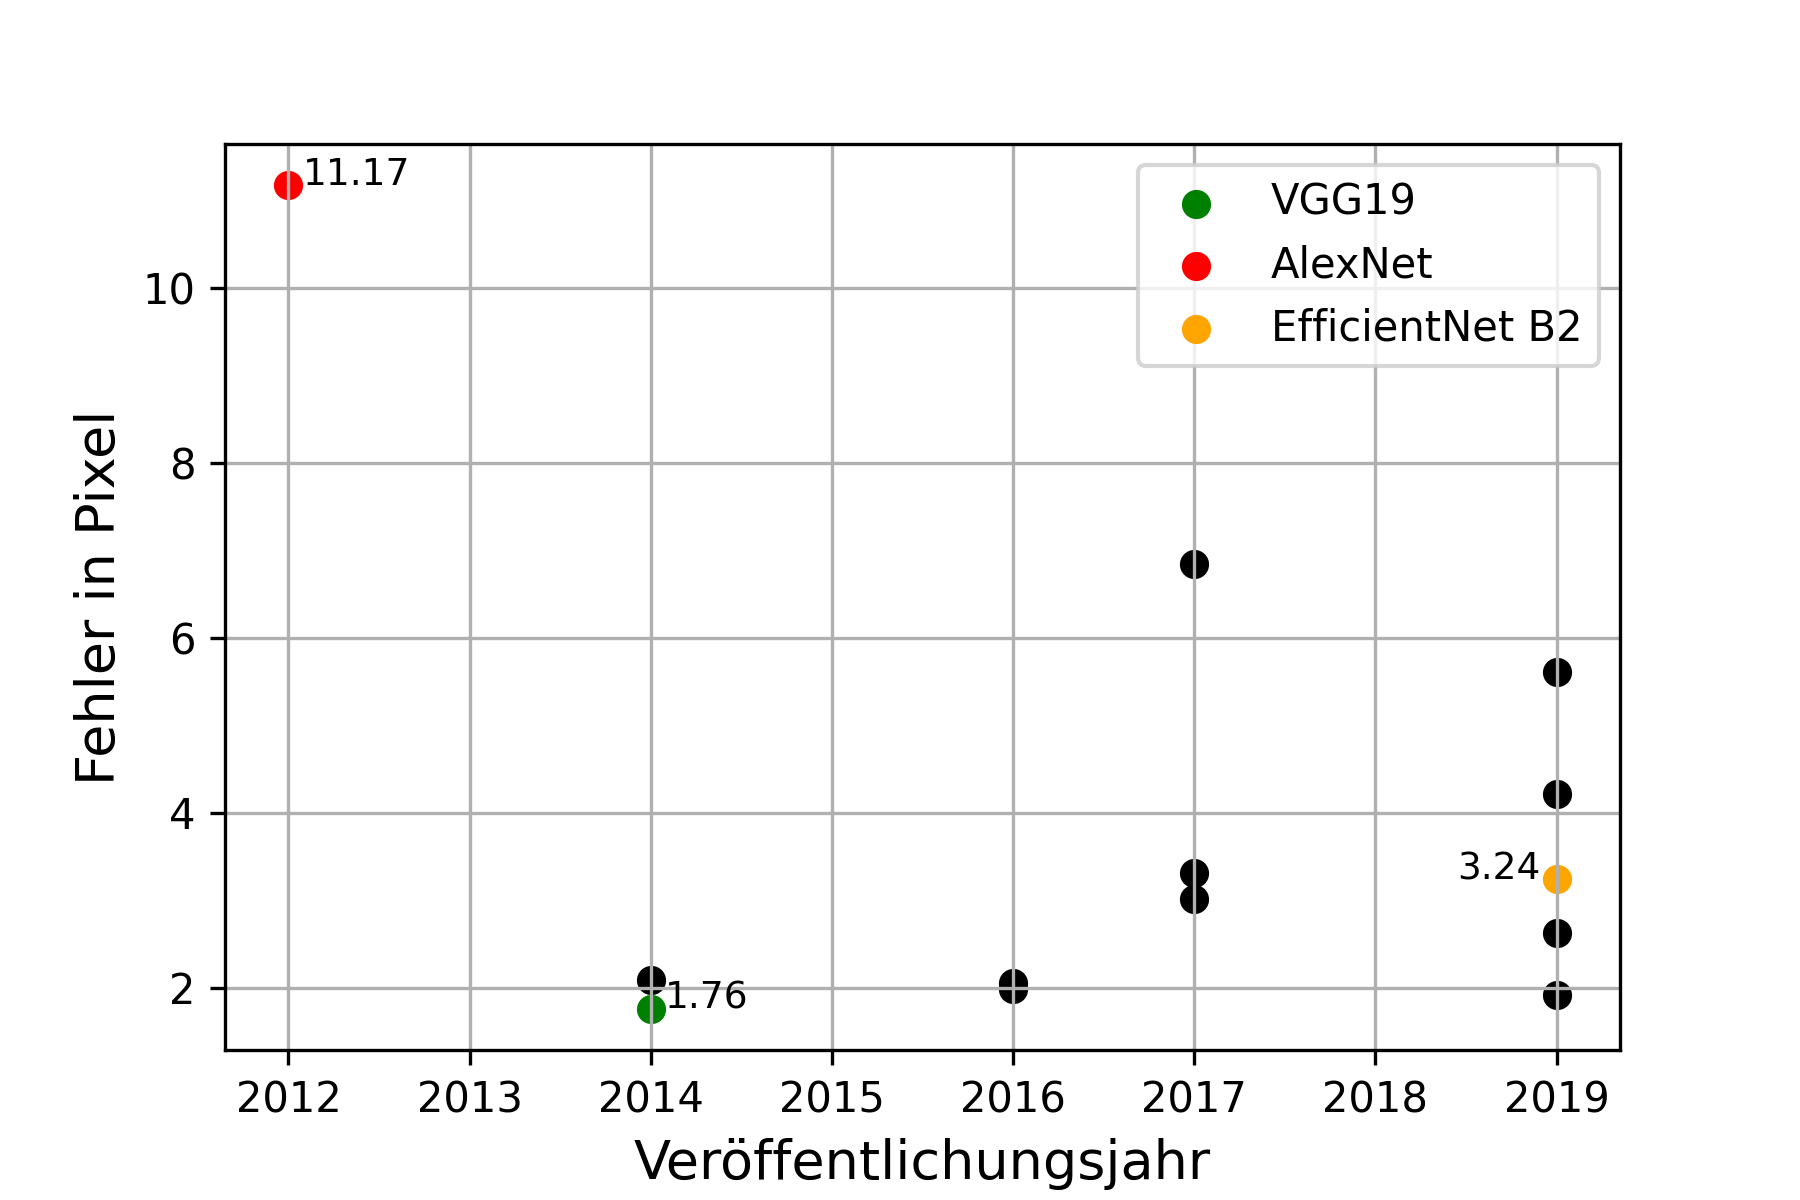
\includegraphics[width=11cm]{98_images/year_error_graph.png}
\caption{Vergleich des Fehlers nach Veröffentlichungsjahr der Netzwerkarchitekturen}
\label{fig:year-error-graph}
\end{figure}

\begin{figure}[h!]
\centering
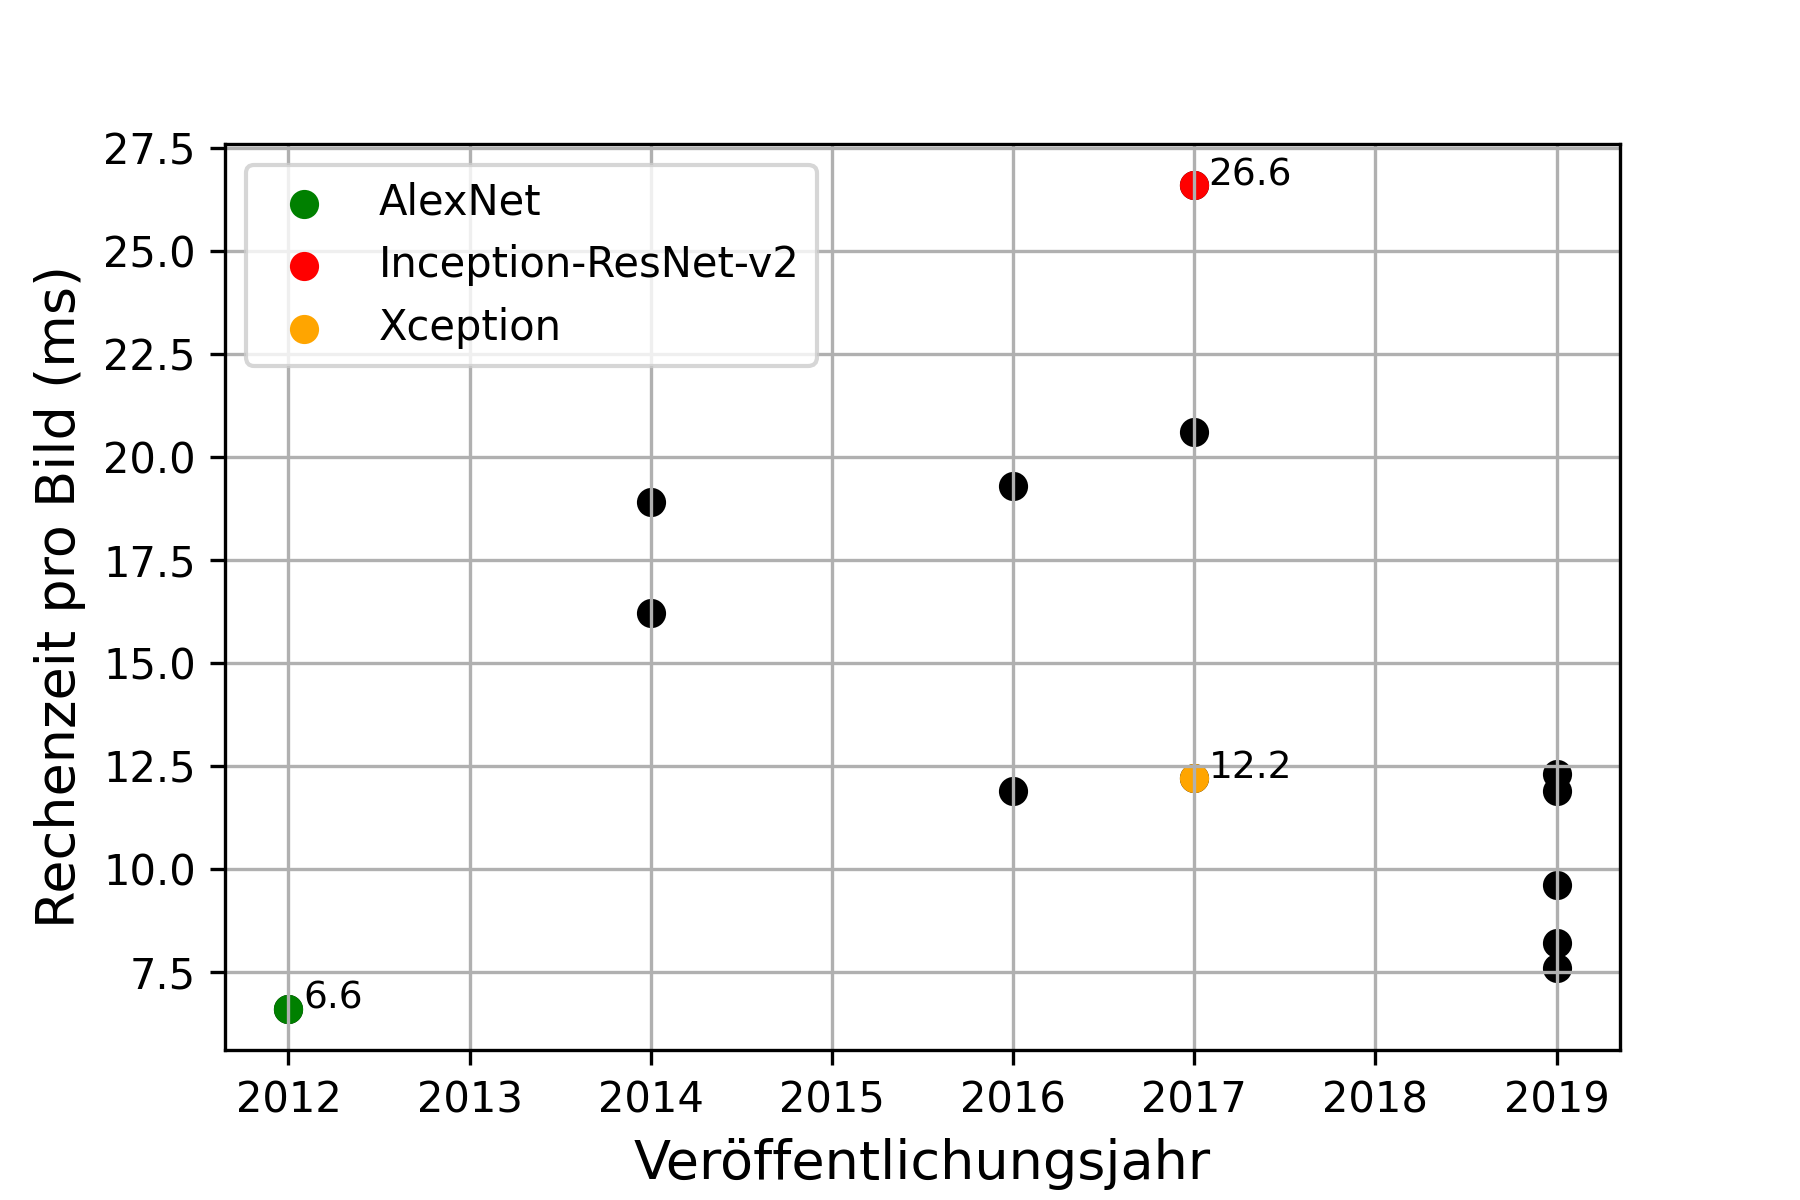
\includegraphics[width=11cm]{98_images/year_time_graph.png}
\caption{Vergleich der Rechenzeit pro Bild nach Veröffentlichungsjahr der Netzwerkarchitekturen}
\label{fig:year-time-graph}
\end{figure}

\mypar Nach Angaben des Industriepartners muss das Gesamtsystem zur Fehlererkennung und -korrektur in der Lage sein, zehn Picks innerhalb einer Sekunde zu inspizieren. Obwohl alle in diesem Abschnitt vorgestellten Werte unter dieser Schranke liegen, muss betrachtet werden, dass dies das Erfassen von Bildern, deren Vorverarbeitung, die Lokalisierung von Picks und weitere Schritte des Verfahrens nicht miteinbezieht.


% Trainingsdauer
\subsection{Trainingsdauer}
Der dritte und letzte Vergleichsfaktor unter den Netzen ist die benötigte Trainingsdauer. Allerdings hat diese keinen Einfluss auf die Leistung der neuronalen Netzwerke. Aufgrund seiner geringen Anzahl an Schichten schneidet hier die AlexNet-Architektur am besten ab. Unter den restlichen Modellen schwankt die Trainingsdauer zwischen zehn und zwanzig Stunden. Eine Übersicht der beim Fehler und Rechenzeit hervorgehobenen Netze, aus den Abschnitten \ref{sec:fehler-sec} und \ref{sec:rechenzeit-label}, ist in Tabelle \ref{Tab:vergleich-netze} aufgezeigt.


% Fehler zu Rechenzeit
\subsection{Fehler zu Rechenzeit}
Da der Fehler und die Rechenzeit die wichtigsten Faktoren sind, wurden diese ebenfalls, wie in Abbildung \ref{fig:time_error_graph} zu sehen, miteinander verglichen. Anhand des Graphens ist ersichtlich, dass das VGG19 zwar den niedrigsten Fehler macht, sich dennoch unter den langsamsten Netzen bei der Vermessung der Picklänge befindet. Im Gegensatz dazu führt das MobileNetV3 large zu einer leicht höheren durchschnittlichen Abweichung von etwa 0,16 Pixel. Dafür wird die Länge eines Picks mehr als doppelt so schnell wie beim VGG19 vermessen. Bei der small Variante der MobileNetV3-Architektur beträgt diese Zeit etwas weniger als bei der large Variante. Allerdings ist der Unterschied beim erzeugten Fehler im Vergleich zum MobileNetV3 large deutlich größer. 

\begin{figure}[h!]
\centering
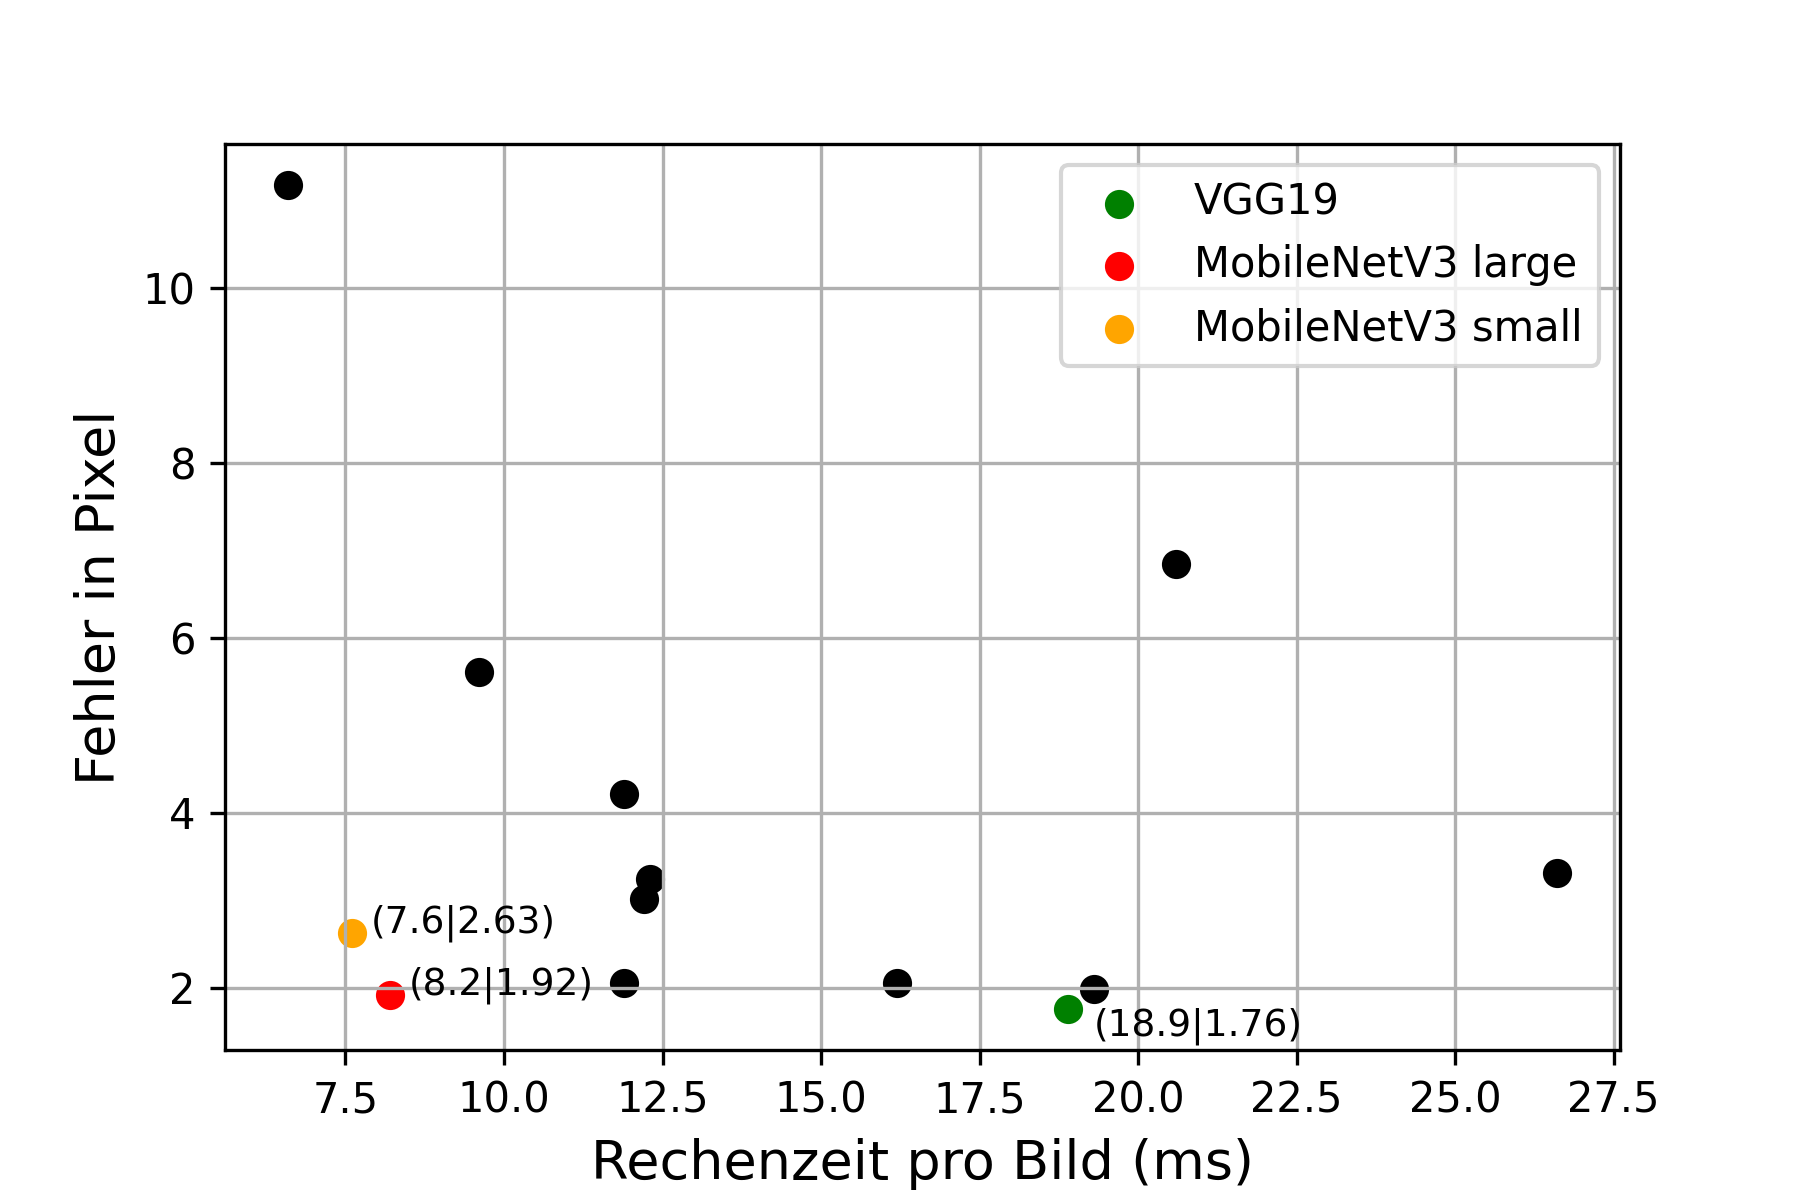
\includegraphics[width=11cm]{98_images/time_error_graph.png}
\caption{Vergleich des Fehlers nach der benötigten Rechenzeit pro Bild}
\label{fig:time_error_graph}
\end{figure}


% Bestimmung der Abweichung
\section{Bestimmung der Abweichung}
Zu Beginn des Flechtvorgangs sind sowohl der Soll-Wert $l_{soll}$ für die Länge der Picks, als auch ein beliebiger Toleranzwert $l_t$ angegeben. Darauffolgend wird, aus der Analyse eines Picks durch ein faltendes neuronales Netz, die vom System gemessene Picklänge ausgegeben, welche dem Ist-Wert $l_{ist}$ entspricht. Somit kann die Abweichung $l_{diff}$ der Netzausgabe durch den Betrag der Differenz zwischen dem Soll- und Ist-Wert wie in Gleichung \ref{eq:abweichung-netz} berechnet werden. 

\begin{equation}\label{eq:abweichung-netz}
l_{diff} = | l_{soll}-l_{ist} |
\end{equation}

\mypar Die Werte der Abweichungen eines Netzes können als Histogramm dargestellt werden. Ein solches Diagramm ist in Abbildung \ref{fig:vgg-histogramm} für das Testen einer trainierten VGG19-Architektur auf den Testdatensatz abgebildet. Für die meisten Bilder beträgt die Abweichung der Netzausgaben weniger als einen Pixel. Da es bei allen Netzen oftmals zu Ausgaben kommt, welche eine große Differenz aufweisen, wurde dies in Abschnitt \ref{sec:fehlerquellen-sec} näher untersucht.

\begin{figure}[h!]
\centering
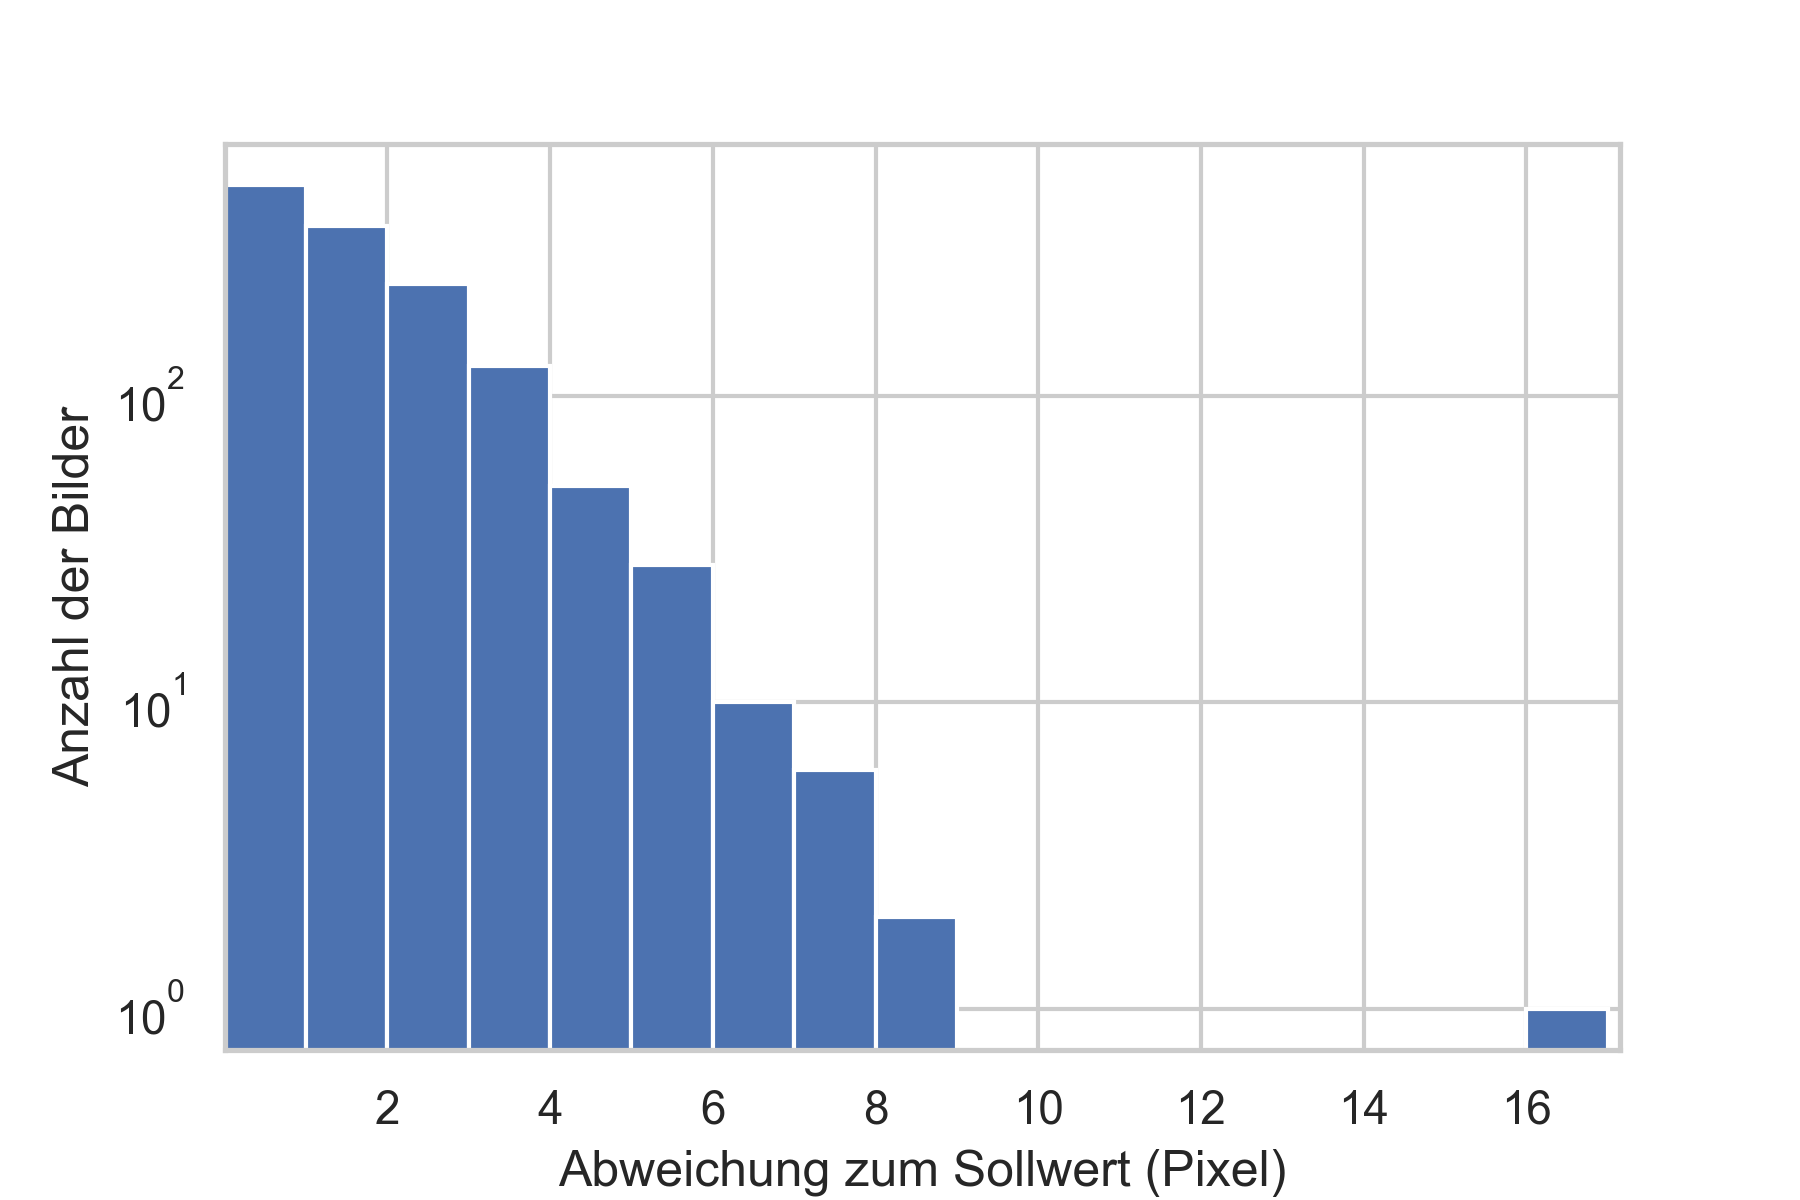
\includegraphics[width=10cm]{98_images/vgg_histogramm.png}
\caption{Aufteilung der Abweichungen bei den Ausgaben eines trainierten VGG19 auf den Testdatensatz}
\label{fig:vgg-histogramm}
\end{figure}

\mypar Werden die Abweichungen der fünf Architekturen mit dem besten Fehler näher betrachtet, wie in Abbildung \ref{fig:best-worst-preds} aufgezeigt, fällt auf, dass ein besserer Fehler nicht mit einem niedrigeren Intervall zwischen der besten und schlechtesten Vermessung zusammenhängt. So liegen sowohl die größten, als auch die niedrigsten Abweichungen beim ResNet101V2 und VGG16 niedriger als bei neuronalen Netzen wie das VGG19 und MobileNetV3 large, welche einen besseren Fehler erzielen. 

\begin{figure}[h!]
\centering
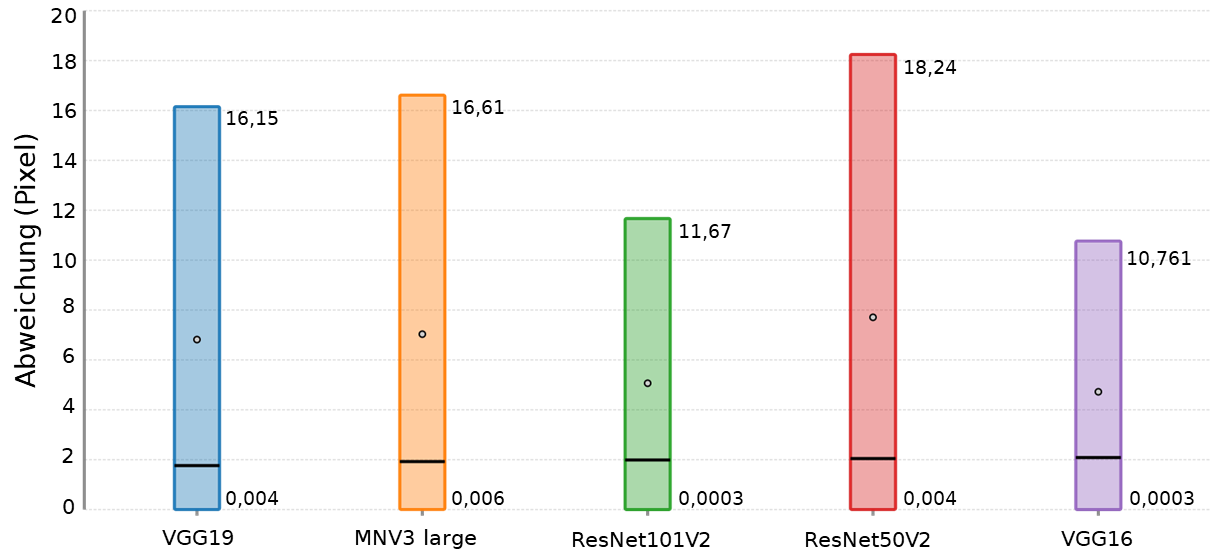
\includegraphics[width=14.5cm]{98_images/best_worst_preds.png}
\caption{Aufteilung der Abweichungen unter den fünf Netzen mit dem besten Fehler}
\label{fig:best-worst-preds}
\end{figure}


% Fehlererkennung
\section{Fehlererkennung}
Die errechnete Abweichung kann mit dem Toleranzwert verglichen werden, um über einen potentiellen Defekt im Stent zu entscheiden. Sollte diese kleiner oder gleich dem Wert der Toleranz $l_t$ wie in Gleichung \ref{eq:abweichung-netz-toleranz} sein, liegt diese noch im Toleranzbereich, sodass der Pick den Qualitätsanforderungen entspricht. Andernfalls entspricht die vom Netz gemessene Picklänge nicht den vorgegebenen Anforderungen, sodass der Pick als fehlerhaft empfunden wird.

\begin{equation}\label{eq:abweichung-netz-toleranz}
l_{diff} \leq l_t
\end{equation}

\mypar Je nachdem wie der Toleranzwert festgelegt wird, wird die Leistung des Systems beeinflusst. Ist dieser zu hoch, werden weniger Defekte gemeldet, wodurch das System weniger falsch negative Ergebnisse anzeigt und die Produktivität gesteigert wird. Auf der anderen Seite können Defekte dadurch übersehen werden, womit die Genauigkeit und Zuverlässigkeit der Überprüfung sinkt. 


% Mögliche Fehlerquellen
\section{Mögliche Fehlerquellen}\label{sec:fehlerquellen-sec}
Im Rahmen dieses Abschnitts sollen Gründe für Abweichungen zwischen den Soll- und Ist-Werten erklärt werden. Für Abweichungen einer hohen Größenordnung wurden zwei Gründe festgestellt. Zum einen sind Teile des mittleren Picks auf einigen Bildern schlecht erkennbar. Im betrachteten Pick aus Abbildung \ref{fig:bilder-abweichungen} links, ist die obere Ecke der Struktur schlecht erkennbar. Aus diesem Bild ergab sich die größte Abweichung mit dem VGG19, nämlich 16,2 Pixel.

\begin{figure}[h!]
\centering
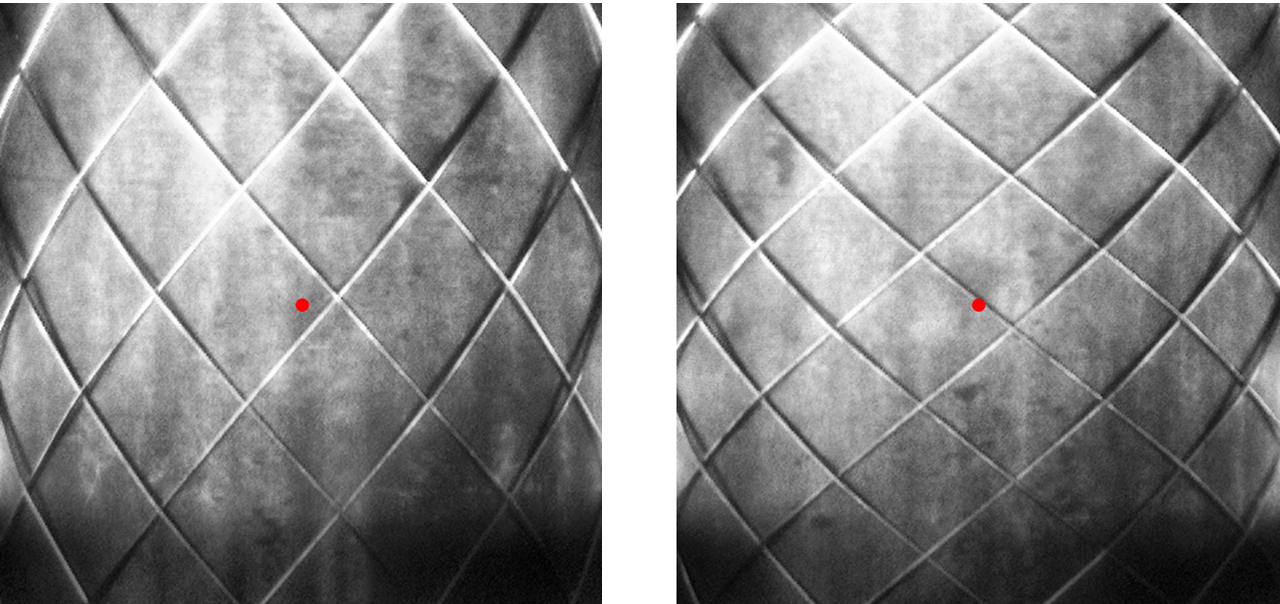
\includegraphics[width=9cm]{98_images/grosse_abweichungen.png}
\caption{Beispiele für Bilder, welche zu großen Abweichungen bei der Netzausgabe geführt haben. Der Mittelpunkt der Bilder ist rot markiert.}
\label{fig:bilder-abweichungen}
\end{figure}

\mypar Der zweite und meist verbreitete Grund ist rechts in Abbildung \ref{fig:bilder-abweichungen} dargestellt. Ein zwischen zwei Picks positionierter Mittelpunkt des Bildes führte oftmals zu großen Abweichungen bei den Netzen.

\mypar Abweichungen einer geringen Größe können aufgrund ungenauer Labels entstehen. In Anbetracht der breiten Anzahl an Bildern, von denen die Labels in Zusammenarbeit erstellt wurden, und dem unvermeidbaren menschlichen Fehler, sind Ungenauigkeiten in den Labels unumgänglich. Somit ist es möglich, dass die Netze zwar die richtigen Eigenschaften der Bilder erlernen, sich aber Abweichungen infolge ungenauer Labels bilden. 


% Bewertung des Systems
\section{Bewertung des Systems}\label{sec:bewertung-system-sec}
Bezogen auf das Projekt Stents4Tomorrow \cite{flechtmaschine} sind drei wichtige Größen für die Genauigkeit des Systems zur automatisierten Korrektur von Fehlern in Stents vorgegeben. Ein optimales System muss in der Lage sein, Picklängen mit einer Genauigkeit von $\pm 0,01$ Millimeter zu berechnen. Bei einer guten Leistung verdoppelt sich dieser Wert und ein ausreichendes Ergebnis bedingt eine Genauigkeit von 0,05 Millimeter. Diese Werte werden als $l_1$, $l_2$ und $l_3$ gekennzeichnet.

\mypar Abbildung \ref{fig:abweichungen-je-toleranz} zeigt den prozentualen Anteil an Bildern aus dem Testdatensatz, welche von unterschiedlichen Netzen bei einen gewissen Toleranzwert richtig vermessen werden. Hierbei sind die drei zuvor erläuterten Vorgaben ebenso im Graphen eingetragen. Hieraus kann abgelesen werden, dass die zwei Netze mit dem besten Fehler, das VGG19 und MobileNetV3, ab einer Toleranz von etwa sieben Pixeln nahe an die 100{\%} kommen. Die aus der Auswahl neueste Architektur, das EfficientNet B2, benötigt etwa 11,5 Pixel. Das AlexNet hingegen erreicht, trotz einer Toleranz von 12 Pixeln, was mehr als einen halben Millimeter entspricht, eine Genauigkeit von ungefähr 65{\%}.

\begin{figure}[h!]
\centering
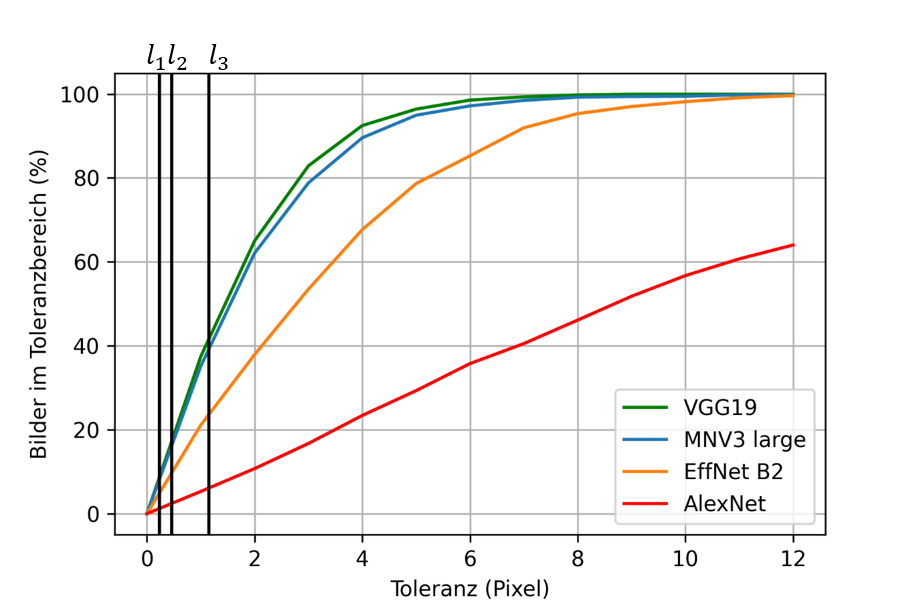
\includegraphics[width=14cm]{98_images/abweichungen_nach_toleranz.png}
\caption{Prozentanteil der Ausgaben mehrerer Netze je nach gesetzter Toleranz. Die drei vorgegebenen Größen $l_1 = 0,23 \text{ Pixel}, l_2 = 0,46 \text{ Pixel und } l_3 = 1,15 \text{ Pixel}$ sind eingezeichnet.}
\label{fig:abweichungen-je-toleranz}
\end{figure}

\mypar Werden diese Ergebnisse nun mit den Zielwerten verglichen, wird deutlich, dass die $l_1$- und $l_2$-Werte aktuell noch nicht erreicht werden können. Die Ak­ku­ra­tes­se des aktuell genauesten Netzes liegt hinsichtlich dieser Werte bei etwa 8,1{\%} und 16,8{\%}. Selbst eine ausreichend gute Vermessung der Picklänge kann aktuell nur in ungefähr 43,3{\%} der Fälle erreicht werden.



